
\documentclass[english,onecolumn]{IEEEtran}
\usepackage[T1]{fontenc}
\usepackage[latin9]{luainputenc}
\usepackage[letterpaper]{geometry}
\geometry{verbose}
\usepackage{amsfonts}
\usepackage{babel}
\usepackage{ulem}

\usepackage{extarrows}
\usepackage[colorlinks]{hyperref}
\usepackage{listings}
\usepackage{xcolor}
\usepackage[ruled,linesnumbered]{algorithm2e}

\usepackage{amsmath,graphicx}
\usepackage{subfigure} 
\usepackage{cite}
\usepackage{amsthm,amssymb,amsfonts}
\usepackage{textcomp}
\usepackage{bm,pifont}
\usepackage{booktabs}
\usepackage{listings}
\usepackage{xparse}
\usepackage{cleveref}
\usepackage{xcolor}
\usepackage[center]{caption}

\definecolor{salmon}{rgb}{1, 0.5020, 0.4471}

\NewDocumentCommand{\codeword}{v}{
\texttt{\textcolor{blue}{#1}}
}

\lstdefinestyle{mystyle}{
    backgroundcolor=\color{backcolour},   
    commentstyle=\color{codegreen},
    keywordstyle=\color{magenta},
    numberstyle=\tiny\color{codegray},
    stringstyle=\color{codepurple},
    basicstyle=\ttfamily\footnotesize,
    breakatwhitespace=false,         
    breaklines=true,                 
    captionpos=b,                    
    keepspaces=true,                 
    numbers=left,                    
    numbersep=5pt,                  
    showspaces=false,                
    showstringspaces=false,
    showtabs=false,                  
    tabsize=2
}

\lstset{style=mystyle}

\providecommand{\U}[1]{\protect\rule{.1in}{.1in}}
\topmargin            -18.0mm
\textheight           226.0mm
\oddsidemargin      -4.0mm
\textwidth            166.0mm
\def\baselinestretch{1.5}


\newtheorem{theorem}{Theorem}[section]
\newtheorem{lemma}[theorem]{Lemma}

\newcommand{\Rbb}{\mathbb{R}}
\newcommand{\Pb}{\mathbf{P}}
\newcommand{\Ib}{\mathbf{I}}
\newcommand{\vb}{\mathbf{v}}
\newcommand{\Ucal}{\mathcal{U}}
\newcommand{\Wcal}{\mathcal{W}}
\newcommand{\Vcal}{\mathcal{V}}
\newcommand{\Rcal}{\mathcal{R}}
\newcommand{\Ncal}{\mathcal{N}}
\newcommand{\bigO}{\mathcal{O}}
\newcommand{\bigS}{\mathcal{S}}
\newcommand{\bA}{{\bf A}}
% \newcommand{\bU}{{\bf U}}
\newcommand{\bV}{{\bf V}}
\newcommand{\bY}{{\bf Y}}
\newcommand{\bX}{{\bf X}}
\newcommand{\bmu}{{\boldsymbol \mu}}
\newcommand{\bSig}{{\boldsymbol \Sigma}}
\newcommand{\bone}{{\boldsymbol 1}}
\newcommand{\bQ}{{\bf Q}}
\newcommand{\bR}{{\bf R}}
\newcommand{\bH}{{\bf H}}
\newcommand{\bU}{{\bf U}}
\newcommand{\bT}{{\bf T}}
\newcommand{\bI}{{\bf I}}
\newcommand{\bq}{{\bf q}}
\newcommand{\bz}{{\bf z}}
\newcommand{\bL}{{\bf L}}
\newcommand{\bx}{{\bf x}}
\newcommand{\bv}{{\bf v}}
\newcommand{\bG}{{\bf G}}
\def\A{\mathbf{A}}
\def\v{\mathbf{v}}

\begin{document}

\begin{center}
	\textbf{\LARGE{SI231 - Matrix Computations, Fall 2020-21}}\\
	{\Large Homework Set \#5}\\
	\texttt{Prof. Yue Qiu and Prof. Ziping Zhao}\\
	\texttt{\textbf{Name:}}   	\texttt{ Ziyi Yu }  		\hspace{1bp}
	\texttt{\textbf{Major:}}  	\texttt{ Bachelor in CS } 	\\
	\texttt{\textbf{Student No.:}} 	\texttt{ 2018533124 }     \hspace{1bp}
	\texttt{\textbf{E-mail:}} 	\texttt{ yuzy@shanghaitech.edu.cn}
\par\end{center}

\noindent
\rule{\linewidth}{0.4pt}
{\bf {\large Acknowledgements:}}
\begin{enumerate}
    \item Deadline: \textcolor{red}{\textbf{2020-12-07 23:59:00}}
    \item Submit your homework at \textbf{Gradescope}.
    Homework \#5 contains two parts, the theoretical part the and the programming part.
    \item About the the theoretical part:
    \begin{enumerate}
            \item[(a)] Submit your homework in \textbf{Homework 5} in gradescope. Make sure that you have correctly select pages for each problem. If not, you probably will get 0 point.
            \item[(b)] Your homework should be uploaded in the \textbf{PDF} format, and the naming format of the file is not specified.
            \item[(c)] No handwritten homework is accepted. You need to use \LaTeX $\,$ in principle.
            \item[(d)] Use the given template and give your solution in English. Solution in Chinese is not allowed. 
        \end{enumerate}
  \item About the programming part:
  \begin{enumerate}
      \item[(a)] Submit your codes in \textbf{Homework 5 Programming part} in gradescope. 
      \item[(b)] When handing in your homework in gradescope, package all your codes into {\sf your\_student\_id+hw4\_code.zip} and upload. In the package, you also need to include a file named {\sf README.txt/md} to clearly identify the function of each file. (\textcolor{blue}{".zip" format package rather than ".rar, .7zip" should be uploaded, solution of the results should be named according to requirements}.)
     \item[(c)] Make sure that your codes can run and are consistent with your solutions.
  \end{enumerate}
  \item \textbf{Late Policy details can be found in the bulletin board of Blackboard.}
\end{enumerate}
\rule{\linewidth}{0.4pt}

\section*{Study Guide}
\noindent
This homework concerns the following topics:
\begin{itemize}
    \item \textbf{Regularization}, see Lecture 8 of Zhao, Lecture 20 of Qiu.
    \item \textbf{SVD computation}, see Lecture 7 of Zhao, Lecture 18 of Qiu. 
    \item \textbf{Iterative methods}, see Lecture 2 of Zhao, Lecture 21 of Qiu. 
    \item \textbf{Application of SVD, PCA}, see Lecture 7 of Zhao, Lecture 19 of Qiu. 
\end{itemize}

\newpage
\section{Least square with regularization}
\noindent\textbf{Problem 1}. 
In this problem, we will learn how to solve LS when there is noise. for some $\lambda>0$, where the term $\lambda||\mathbf{x}||^{k}_{k}$ is added to improve the system conditioning, thereby attempting to reduce noise sensitivity. Usually, we set $k=1$ which is called $\ell$1 regularization, or set $k=2$ which is called $\ell$2 regularization. 

\noindent $\ell$1 regularized LS:
\begin{equation}
    \mathbf{x_{LS}}=\min_{\mathbf{X}\in\mathbf{\Rbb}^{n}}f(\mathbf{x}), \quad f(\mathbf{x})=||\mathbf{Ax-y}||^{2}_{2}+\lambda||\mathbf{x}||_{1}
\end{equation}
\noindent $\ell$2 regularized LS:
\begin{equation}
    \mathbf{x_{LS}}=\min_{\mathbf{X}\in\mathbf{\Rbb}^{n}}f(\mathbf{x}),\quad f(\mathbf{x})=||\mathbf{Ax-y}||^{2}_{2}+\lambda||\mathbf{x}||^{2}_{2}
\end{equation}

Write programs to solve the regularized least square problem, any programming language is suitable. where $\mathbf{A} \in \Rbb^{m \times n}$ is a matrix representing the predefined data set with $m$ data samples of $n$ dimensions ($m$=1000, $n$=210), and $\mathbf{y} \in \Rbb^m$ represents the labels. The data samples are provided in the "data.txt" file, and the labels are provided in the "label.txt" file, you are supposed to load the data before solving the problem. In this problem, we set $\lambda=0.1$ for two algorithms.
\begin{enumerate}
    \item (\textcolor{blue}{\textbf{8 points}}) Solve $\ell$1 regularized LS using Majorization-Minimization method, we set $c=1e+5$ in this problem. The Majorization-Minimization method for solving problem updates $ {\bf x}$ as
    $$
        {\bf x^{(k+1)}} = \mathbf{soft}(\frac{1}{c}\mathbf{A^{T}}(\mathbf{y}-\mathbf{Ax^{(k)}})+\mathbf{x^{(k)}},\lambda/c),
    $$
 where $\mathbf{soft}$ is called the soft-thresholding operator and is defined as follows: if $\mathbf{z=soft(x,\sigma)}$, then $z_{i}=sign(x_{i})\max\{|x_{i}|-\sigma,0\}$.
    \item (\textcolor{blue}{\textbf{8 points}}) Solve $\ell$2 regularized LS using gradient descent method. The gradient descent method for solving problem updates $ {\bf x}$ as
    $$
        {\bf x} = {\bf x} - \gamma \cdot \nabla_{{\bf x}} f(\mathbf{x}),
    $$
 where $\gamma$ is the step size of the gradient decent methods. We suggest that you can set $\gamma=1e-5$. 
    \item (\textcolor{blue}{\textbf{4 points}}) Compare two methods above. 
    \begin{enumerate}
        \item[(a)] compare L0 norm (the number of non-zero elements) of $\mathbf{x_{LS}}$ computed by above two algorithms;
        \item[(b)] Compare the loss $||\mathbf{Ax-y}||^{2}_{2}$ for results $\mathbf{x}=\mathbf{x_{LS}}$ of above two algorithms.
    \end{enumerate}
\end{enumerate}

\noindent\textbf{Remarks: }
\begin{itemize}
    \item The solution of the two methods should be printed in files named "sol1.txt" and "sol2.txt" and submitted in gradescope.  The format should be same as the input file (210 rows plain text, each rows is a dimension of the final solution).
    \item Make sure that your codes are executable and are consistent with your solutions.
\end{itemize}

\noindent
\textbf{Solution.}
\begin{enumerate}
    \item[3)] \begin{enumerate}
        \item[(a)] L0 norm: \begin{itemize}
            \item Majorization-Minimization method: 210
            \item gradient decent method: 210
        \end{itemize}
        \item[(b)] loss $||\mathbf{Ax-y}||^{2}_{2}$
        \begin{itemize}
            \item Majorization-Minimization method: 2945.7750079902967
            \item gradient decent method: 2945.5282378018974
        \end{itemize}
    \end{enumerate}
\end{enumerate}


\newpage
\section{Computations of SVD}
\noindent\textbf{Problem 2}.
In this problem you will see singular value stability and discover computation of SVD.
\begin{enumerate}
    \item (\textcolor{blue}{\textbf{4 points}}) Consider a $4 \times 4$ matrix
    \[
	\mathbf{A} = \begin{bmatrix}
		0& 1&0&0 \\
		0&0&2&0\\
		0&0&0&3\\
		\frac{1}{6000}&0&0&0
	\end{bmatrix}\,,
	\]
	find its singular values and eigenvalues. In this sub-problem you can use eigenvalue decomposition ('eig') and singular value decomposition function ('svd') in Matlab or Python.
	\item (\textcolor{blue}{\textbf{8 points}}) Compute the SVD decomposition of a $3 \times 2$ matrix by \Cref{alg:svd}
	\[
	\mathbf{B} = \begin{bmatrix}
		3& 2 \\
		1&4  \\
		\frac{1}{2}&\frac{1}{2}
	\end{bmatrix}\,.
	\]
Are the results right? If not, can you get the correct answer through the results of \Cref{alg:svd}? In this sub-problem you can use the eigenvalue decomposition ('eig') and QR decomposition function ('qr') in Matlab or Python.
\item (\textcolor{blue}{\textbf{8 points}}) Consider an $m\times m$ upper triangular matrix with 0.1 on the main diagonal and 1 everywhere above the diagonal. Find the smallest singular value through the singular value decomposition function ('svd') and \cref{alg:svd}. You are required to plot two curves on a log scale for $m=1,\dots,30$ and show which one is the desired result.
\end{enumerate}

\begin{algorithm}[htbp]
\SetKwInOut{Input}{Input}\SetKwInOut{Output}{Output}
\caption{SVD Decomposition by $\mathbf{A}^T\mathbf{A}$}
\label{alg:svd}
\SetAlgoLined
\Input{Thin matrix A}
Form $\mathbf{A}^T\mathbf{A}$.\\
Compute the eigenvalue decomposition $\mathbf{A}^T\mathbf{A}$=$\mathbf{V}^T\mathbf{\Lambda V}$.\\
Let $\mathbf{\Sigma}$ be an m$\times$n diagonal matrix with diagonal entries being the nonnegative square root of diagonal entries of $\mathbf{\Lambda}$.\\
Solve the system $\mathbf{U\Sigma} = \mathbf{AV} $for orthogonal matrix $\mathbf{U}$ (e.g., via QR factorization). \\
\Output{$\mathbf{U}, \mathbf{\Sigma}, \mathbf{V}$.}

\end{algorithm}
{\bf Remarks}
\begin{enumerate}
    \item Singular values cannot be negative.
    \item Please show your result and insert figures in your PDF.
\end{enumerate}

\noindent
\textbf{Solution.}
\begin{enumerate}
    \item[1)] \begin{itemize}
        \item eigen values: $\lambda_1 = -1.77827941e-01+0.j \,, \quad$  $\lambda_2 = -5.55111512e-17+0.17782794j \,, \quad$ \\ $\lambda_3 = -5.55111512e-17-0.17782794j \,, \quad$ $\lambda_4 = 1.77827941e-01+0.j \,, \quad$
        \item singular values: $\sigma_1 = 3.00000000e+00 \,, \quad $ $\sigma_2 = 2.00000000e+00 \,, \quad $ $\sigma_3 = 1.00000000e+00 \,, \quad $ $\sigma_4 = 1.66666667e-04 \,, \quad $
    \end{itemize}
    \begin{figure}[htbp]
        \centering
        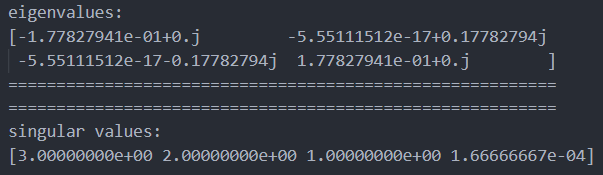
\includegraphics[width=1\textwidth]{p2_1.png}
        \caption{eigenvalues and singular values for problem 1)}
        \label{fig.p2_1}
    \end{figure}
    \item[2)] The result without modification: $$\bm{U}=\begin{bmatrix}
        -0.75696315 & -0.63643976 & -0.14815944 \\
        0.64840237 & -0.75969424 & -0.04938648 \\
        -0.08112435 & -0.13345068 & 0.9877296 \\
    \end{bmatrix}$$ $$\bm{\Sigma} = \begin{bmatrix}
        5.16279912 & 0. \\
        0. & 1.96099599\\
        0. &  0.        
    \end{bmatrix}$$ $$\bm{V} = \begin{bmatrix}
        -0.84806357 & 0.5298945 \\
        0.5298945 &  0.84806357
    \end{bmatrix}$$
    The result given by algorithm \ref{alg:svd} is not right, since the QR factorization is not unique for $\bm{AV}$.
    We can get the desired results if we pose basic row/column transformations on $\bm{U}$ and $\bm{V}$.\\
    The result with modification:
    $$\bm{U}=\begin{bmatrix}
        -0.63643976 &  0.75696315 & -0.14815944\\
        -0.75969424 & -0.64840237 & -0.04938648\\
        -0.13345068 &  0.08112435 & 0.9877296\\
    \end{bmatrix}$$ $$\bm{\Sigma} = \begin{bmatrix}
        5.16279912 & 0. \\
        0. & 1.96099599\\
        0. &  0.        
    \end{bmatrix}$$ $$\bm{V} = \begin{bmatrix}
        -0.5298945 & -0.84806357\\
        0.84806357 & -0.5298945
    \end{bmatrix}$$
    The above decomposition is easily verified to be our desired result.
    \newpage
    \item[3)]  To be more specific, I draw the 2 curves separately, then put them together.
    \begin{figure}[htbp]
        \begin{minipage}[t]{0.33\linewidth} 
            \centering
            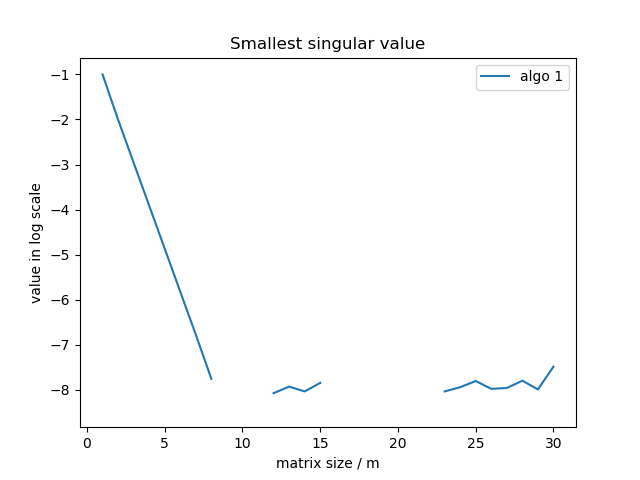
\includegraphics[width=1\textwidth]{p2_3_algo1.png}
            \caption{smallest singular value from algorithm \ref{alg:svd}}
            \label{fig.p2_3_algo1}
        \end{minipage}
        \begin{minipage}[t]{0.33\linewidth}
            \centering
            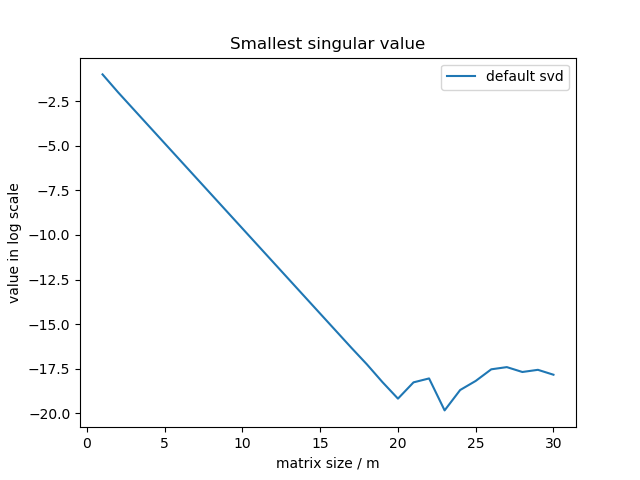
\includegraphics[width=1\textwidth]{p2_3_def.png}
            \caption{smallest singular value from default svd}
            \label{fig.p2_3_def}
        \end{minipage}
        \begin{minipage}[t]{0.33\linewidth}
            \centering
            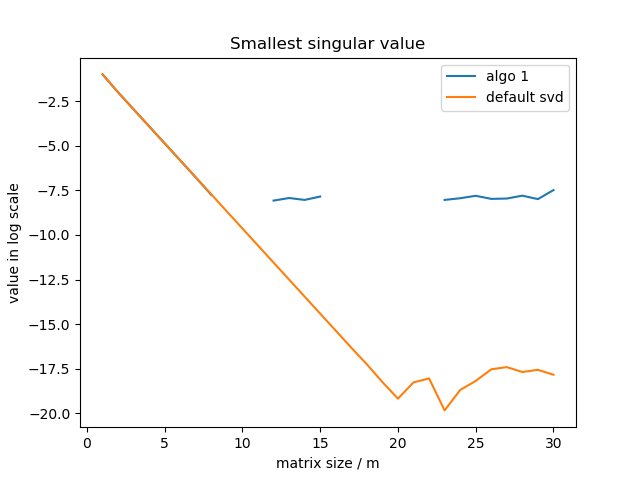
\includegraphics[width=1\textwidth]{p2_3_together.png}
            \caption{smallest singular value}
            \label{fig.p2_3_together}
        \end{minipage}
    \end{figure}
    \\Obviously, the default svd is what we need, since algorithm \ref{alg:svd} gives an unstable svd decomposition.
\end{enumerate}

\clearpage
\newpage
\section{Iterative methods.}
\noindent\textbf{Problem 3}.
In this problem, you will learn how to implement the iterative methods, Jacobi, Gauss-Seidel and SOR Methods to solve the linear equation $\mathbf{b}=\mathbf{Ax}$, and compare the convergence of these methods. 
"A1.txt", "A2.txt","b1.txt", "b2.txt","x1.txt", "x2.txt" is the data of the $\mathbf{b}, \mathbf{x}, \mathbf{A}$ with different size (10 and 1000 respectively).
\begin{algorithm}
	\caption{Iterations method}
	\label{algo:Jacobi}
    \LinesNumbered
	\KwIn{A starting point $\mathbf{x}^{0}$, maximum iterations $N$, error bound $\mathrm{eps}$}
    \KwOut{Solution $\mathbf{x}$ of $\mathbf{Ax}=\mathbf{b}$}
	\For{$k=0,1,2,\dots,N$}{
	    \textbf{update} $\mathbf{x}^k$ to obtain $\mathbf{x}^{k+1}$ \tcp*{Use one of the three iteration methods}
        \If{$\|\mathbf{x}^{k+1}-\mathbf{x}^{k}\|_2< \mathrm{eps}$ }{
            \textbf{break}\;
        }
    }
\end{algorithm}

Suppose $\mathbf{x}\in\mathbb{R}^{n}$, $\mathbf{A}=[a_{ij}]\in\mathbb{R}^{n\times n}$ and $\mathbf{b}=(b_i)\in\mathbb{R}^{n}$.

Each iteration method uses different updates:

For Jacobi Iteration, 
\begin{equation*}
    x_i^{k+1} = (b_i - \sum_{i \neq j} a_{ij}x_j^k) / a_{ii} \quad \text{for }\ i = 1,\dots, n,
\end{equation*}

For Gauss-Seidel Iteration, 
\begin{equation*}
    x_i^{k+1} = (b_i - \sum_{j > i} a_{ij}x_j^{k+1} - \sum_{j < i} a_{ij}x_j^{k}) / a_{ii}, \quad \text{for }\ i = 1,\dots, n,
\end{equation*}

For SOR Iteration with relaxation factor $\omega$, 
\begin{equation*}
    x_i^{k+1} = (1-\omega) x_i^{k} + \omega \left(b_i - \sum_{j>i} a_{ij}x_j^{k+1} - \sum_{j<i} a_{ij}x_j^{k}\right) / a_{ii}, \quad \text{for }\ i = 1,\dots, n.
\end{equation*}

\textbf{Remarks:}
\begin{enumerate}
    \item (\textcolor{blue}{\textbf{8 points}}) Implement the Jacobi Iteration and Gauss-Seidel Iteration methods.
    \item (\textcolor{blue}{\textbf{8 points}}) Implement the SOR Iteration method, tune the relaxation factor $\omega$ to achieve high convergence rate and plot the curve of number of iterations v.s. the value of $\omega$.
    \item (\textcolor{blue}{\textbf{4 points}}) Plot the error $\|\mathbf{x}_{\mathrm{true}} - \mathbf{x}^k\|_2$ for $k=1,2,\dots,N$, analyze the convergence rate and the final error of three methods.
\end{enumerate}
Note: The value of the ``eps'' in Terminal condition should not be too large!



\noindent
\textbf{Solution.}
\newpage
\begin{enumerate}
    \item[2)]
    \begin{figure}[htbp]
        \begin{minipage}[t]{0.5\linewidth} 
            \centering
            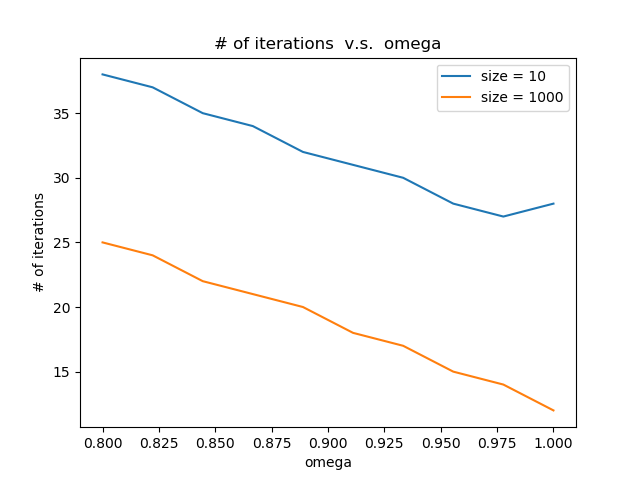
\includegraphics[width=1\textwidth]{p3_2.png}
            \caption{number of iterations v.s. $\omega$ (in a narrow range)}
            \label{fig.p3_2}
        \end{minipage}
        \begin{minipage}[t]{0.5\linewidth}
            \centering
            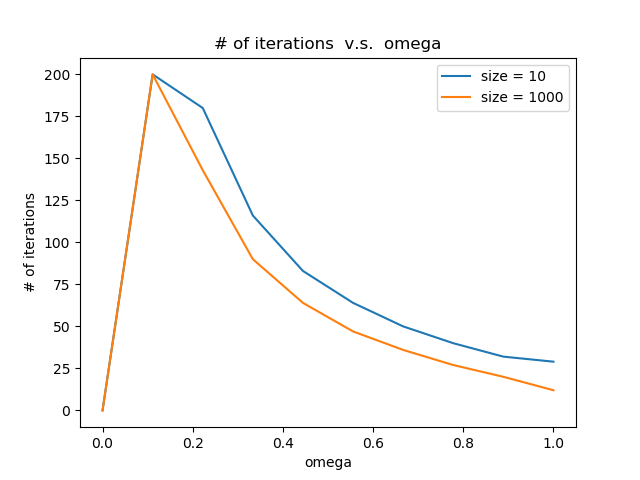
\includegraphics[width=1\textwidth]{p3_2_general.png}
            \caption{number of iterations v.s. $\omega$ (in a wide range)}
            \label{fig.p3_2_general}
        \end{minipage}
    \end{figure}
    It seems from figure \ref{fig.p3_2} and figure \ref{fig.p3_2_general} that, $\omega$ is best around 1 in both cases, which suggests SOR iteration is really close to Gauss-Seidel Iteration.
    \item[3)] 
    \begin{figure}[htbp]
        \begin{minipage}[t]{0.5\linewidth} 
            \centering
            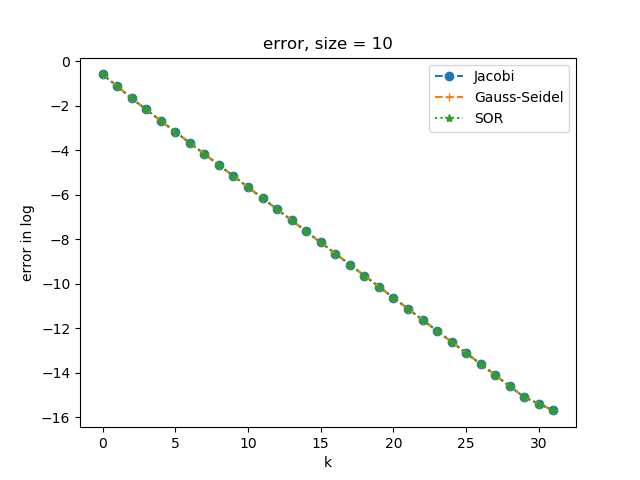
\includegraphics[width=1\textwidth]{p3_3_10.png}
            \caption{error in log scale for size = 10}
            \label{fig.p3_3_10}
        \end{minipage}
        \begin{minipage}[t]{0.5\linewidth}
            \centering
            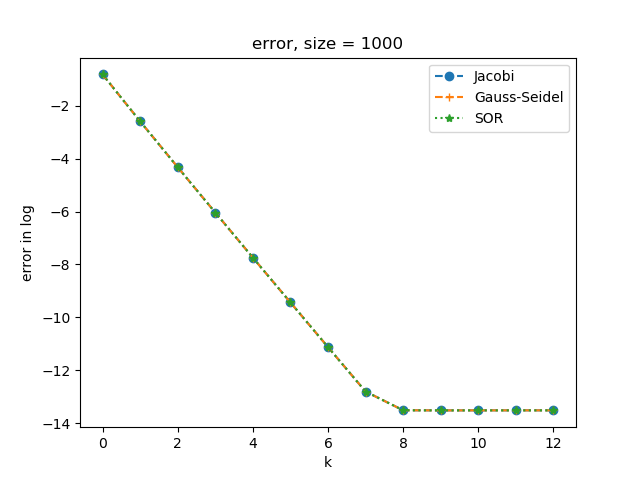
\includegraphics[width=1\textwidth]{p3_3_1000.png}
            \caption{error in log scale for size = 1000}
            \label{fig.p3_3_1000}
        \end{minipage}
    \end{figure}
    The results in figure \ref{fig.p3_3_10} and figure \ref{fig.p3_3_1000} suggest the three methods in fact yields really similar convergence rates and errors.
\end{enumerate}


\newpage
\section{Application of SVD}
\noindent\textbf{Problem 4}.
In this problem you will see one of the application of SVD, what is doing face recognition on Yale B dataset. Here we will only use $4$ individuals under $15$ relatively brighter different illumination conditions.

\begin{figure}[h]
    \centering
    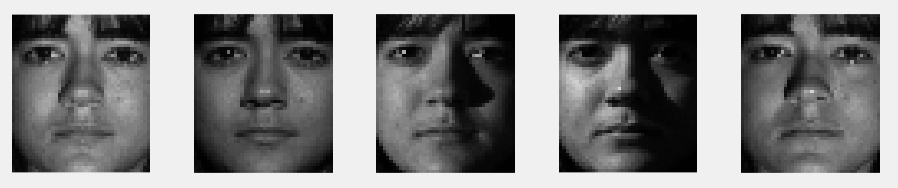
\includegraphics{figures/example_face.png}
    \caption{Face images of one individual under 5 different illumination conditions in the extended YaleB dataset. All images are frontal faces.}
    \label{fig:my_label}
\end{figure}
\vspace{-0.3cm}
Face recongition is an area of computer vision in which low-dimensional linear models such as principal component analysis (PCA) and its variations have been popular tools for capturing the variability of face images. And it has been shown that PCA can be solved by SVD optimally. In the following questions you will see how \Cref{Alg:PCA} can be used.

\vspace{0.5cm}
\begin{algorithm}[H]
\textbf{Parameters}:\\
$\bX$: \quad $D\times N $ data matrix.\\
$d$: \quad Number of principal components.\\
\textbf{Returned values}:\\
$\bmu$: \quad Mean of the data.\\
$\bU$: \quad Orthonormal basis for the subspace.\\
$\bY$: \quad Low-dimensional representation( or principal components).\\
\textbf{Description}:\\
Compute the SVD of the data matrix $\bX - \bmu \bone^T = \bU \bSig \bV^T$.\\
Sort the singular values in descending order, choose the first $d$ singular values and the corresponding $d$ left singular vectors $\bU_d$.\\
Find the $d$ principal components $\bY = \bU_d^T(\bX - \bmu \bone^T)$
\caption{[$\bmu, \bU, \bY$] = PCA\_via\_SVD($\bX,d$) }
\label{Alg:PCA}
\end{algorithm}
\vspace{0.5cm}

The principal bases $\bU$ estimated by PCA are also known as the \textit{eigenfaces} in the computer vision literature. The first eigenface is the left singular vector corresponding to the largest singular value, the second eigenface is the left singular vector corresponding to the second largest singular value and so on.

\begin{enumerate}
    \item (\textcolor{blue}{\textbf{4 points}}) Apply PCA in \Cref{Alg:PCA} with $d = 10$ to individual 4\footnote{you can use the images or the mat file in data1 folder}. Plot the mean face $\bmu$, the first eigenface, the second eigenface, the third eigenface and the tenth eigenface. Describe what you have observed.
    \item (\textcolor{blue}{\textbf{8 points}}) Apply PCA in \Cref{Alg:PCA} with $d = 10$ to the Training Set. 
    \begin{enumerate}
        \item Plot the mean face, the first eigenface, the second eigenface, the third eigenface and the tenth eigenface.
        \item Plot the sorted singular values.
        \item Project the Test Set onto the face subspace given by PCA, that is $\bY_{test} = \bU_d^T(\bX_{test}-\bmu \bone^T)$. Compute the projected faces, that is $\text{Proj}(\bX_{test}) = \bmu \bone^T + \bU_d\bY_{test}$. Then choose one projected face for each individual and plot them. And show those projected faces for $d = 2$ again.
    \end{enumerate} 
    \item (\textcolor{blue}{\textbf{8 points}}) Classify these test faces using 1-nearest-neighbor, that is, label an image $x$ as corresponding to individual $i$ if its projected image $y$ is closest to one of projected training image $y_j$ of individual $i$\footnote{we use $\ell_2$ norm as the distance measurement: $ \|y-y_j\|_2$}. Report the percentage of incorrectly classified face images for $d = 2,...,8$ and put them into the following table. Which value of $d$ gives the best recognition performance?
    \begin{table}[h]
        \centering
        \caption{Summary of errors}
        \begin{tabular}{c|c|c|c|c|c|c|c}
        \# eigenvectors& 2 & 3& 4 & 5 & 6 & 7 & 8 \\ 
        \hline
            error & 0.55 & 0.35 & 0.3 & 0.25 & 0.1 & 0 & 0 
        \end{tabular}
        \label{tab:my_label}
    \end{table}
\end{enumerate}
{\bf Remarks:}
\begin{enumerate}
    \item Data are provided in two forms: images and mat data. You only need to use one of them. 
    \item $10$ images for each individuals in the training data, and $5$ images for each individuals in the test data. All images are of the same size $48\times 42$.
    \item In mat file \textbf{all\_data.mat}, \textbf{data\_train} and \textbf{data\_test} are the matrices of training data and test data where each column is the column stack of an image\footnote{the column stack of an image matrix $\bX\in \Rbb^{m\times n}$ is denoted by $x = [X_{11},X_{21},X_{31},...,X_{mn}]^T\in\Rbb^{mn}$}, \textbf{Y\_label\_train} and \textbf{Y\_label\_test} are ground truth labels.
    \item `Plot the mean face or eigenface' means you should reshape the vector to the size of image and show it.
    \item Recommend to use truncated(thin) SVD for fast implementation.
    \item Please \textbf{insert your figures in your PDF}.
\end{enumerate}

\noindent
\textbf{Solution.}
\begin{enumerate}
    \newpage
    \item [1)] See figure \ref{fig.p4_1}
    \begin{figure}[htbp]
        \subfigure[1st eigenface]{
            \begin{minipage}[t]{0.2\linewidth} 
            \centering
            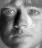
\includegraphics[width=1\textwidth]{figures/p4/problem1/eigenface_1.jpg}
            \end{minipage}
        }
        \subfigure[2nd eigenface]{
            \begin{minipage}[t]{0.2\linewidth} 
            \centering
            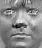
\includegraphics[width=1\textwidth]{figures/p4/problem1/eigenface_2.jpg}
            \end{minipage}
        }
        \subfigure[3rd eigenface]{
            \begin{minipage}[t]{0.2\linewidth} 
            \centering
            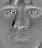
\includegraphics[width=1\textwidth]{figures/p4/problem1/eigenface_3.jpg}
            \end{minipage}
        }
        \subfigure[10th eigenface]{
            \begin{minipage}[t]{0.2\linewidth} 
            \centering
            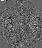
\includegraphics[width=1\textwidth]{figures/p4/problem1/eigenface_10.jpg}
            \end{minipage}
        }
        \subfigure[mean face]{
            \begin{minipage}[t]{0.2\linewidth} 
            \centering
            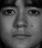
\includegraphics[width=1\textwidth]{figures/p4/problem1/meanface.jpg}
            \end{minipage}
        }
        \caption{mean face and eigenfaces for problem 1}
        \label{fig.p4_1}
    \end{figure} 

    \newpage
    \item [2)] \begin{enumerate}
        \item [a)] see Figure \ref{fig.p4_2_1}
        \begin{figure}[htbp]
            \subfigure[1st eigenface]{
                \begin{minipage}[t]{0.2\linewidth} 
                \centering
                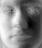
\includegraphics[width=1\textwidth]{figures/p4/problem2/eigenface_1.jpg}
                \end{minipage}
            }
            \subfigure[2nd eigenface]{
                \begin{minipage}[t]{0.2\linewidth} 
                \centering
                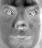
\includegraphics[width=1\textwidth]{figures/p4/problem2/eigenface_2.jpg}
                \end{minipage}
            }
            \subfigure[3rd eigenface]{
                \begin{minipage}[t]{0.2\linewidth} 
                \centering
                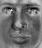
\includegraphics[width=1\textwidth]{figures/p4/problem2/eigenface_3.jpg}
                \end{minipage}
            }
            \subfigure[10th eigenface]{
                \begin{minipage}[t]{0.2\linewidth} 
                \centering
                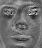
\includegraphics[width=1\textwidth]{figures/p4/problem2/eigenface_10.jpg}
                \end{minipage}
            }
            \subfigure[mean face]{
                \begin{minipage}[t]{0.2\linewidth} 
                \centering
                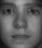
\includegraphics[width=1\textwidth]{figures/p4/problem2/meanface.jpg}
                \end{minipage}
            }
            \caption{mean face and eigenfaces for problem 2}
            \label{fig.p4_2_1}
        \end{figure}
        
        \newpage
        \item [b)] see Figure \ref{fig.p4_2_2}
        
        \begin{figure}[htbp]
                \centering
                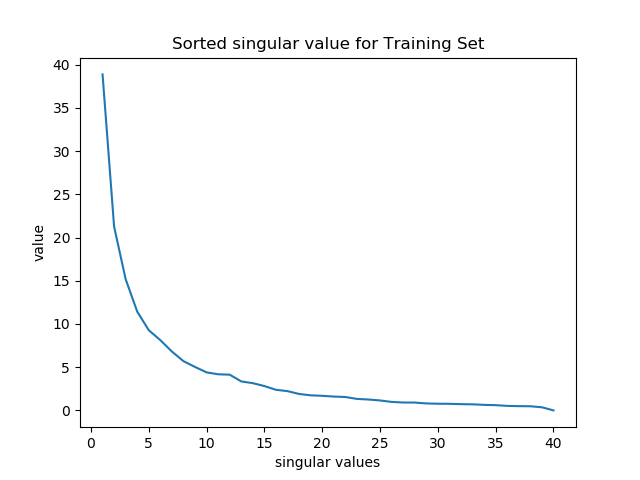
\includegraphics[width=1\textwidth]{p4_2_b.png}
                \caption{sorted singular values}
                \label{fig.p4_2_2}
        \end{figure}

        \newpage
        \item [c)] see Figure \ref{fig.p4_2_3}
        \begin{figure}[htbp]
            \subfigure[id = 0, d = 2]{
                \begin{minipage}[t]{0.22\linewidth} 
                \centering
                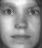
\includegraphics[width=1\textwidth]{figures/p4/problem2/projectface_0_d-2.jpg}
                \end{minipage}
            }
            \subfigure[id = 0, d = 10]{
                \begin{minipage}[t]{0.22\linewidth} 
                \centering
                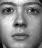
\includegraphics[width=1\textwidth]{figures/p4/problem2/projectface_0_d-10.jpg}
                \end{minipage}
            }
            \subfigure[id = 5, d = 2]{
                \begin{minipage}[t]{0.22\linewidth} 
                \centering
                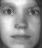
\includegraphics[width=1\textwidth]{figures/p4/problem2/projectface_5_d-2.jpg}
                \end{minipage}
            }
            \subfigure[id = 5, d = 10]{
                \begin{minipage}[t]{0.22\linewidth} 
                \centering
                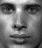
\includegraphics[width=1\textwidth]{figures/p4/problem2/projectface_5_d-10.jpg}
                \end{minipage}
            }
            \subfigure[id = 10, d = 2]{
                \begin{minipage}[t]{0.22\linewidth} 
                \centering
                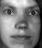
\includegraphics[width=1\textwidth]{figures/p4/problem2/projectface_10_d-2.jpg}
                \end{minipage}
            }
            \subfigure[id = 10, d = 10]{
                \begin{minipage}[t]{0.22\linewidth} 
                \centering
                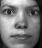
\includegraphics[width=1\textwidth]{figures/p4/problem2/projectface_10_d-10.jpg}
                \end{minipage}
            }
            \subfigure[id = 15, d = 2]{
                \begin{minipage}[t]{0.22\linewidth} 
                \centering
                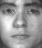
\includegraphics[width=1\textwidth]{figures/p4/problem2/projectface_15_d-2.jpg}
                \end{minipage}
            }
            \subfigure[id = 15, d = 10]{
                \begin{minipage}[t]{0.22\linewidth} 
                \centering
                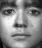
\includegraphics[width=1\textwidth]{figures/p4/problem2/projectface_15_d-10.jpg}
                \end{minipage}
            }
            \caption{projected faces for d=2 and d=10}
            \label{fig.p4_2_3}
        \end{figure}
    \end{enumerate}
    \item [3)] See table \ref{tab:my_label}. The performance of this algorithm evolves as d rise up. Obviously, when $d$ is larger than 7 (d = 7,8), the method gives perfect performance for this test set.
\end{enumerate}


\clearpage
\newpage
\noindent\textbf{Problem 5}.
In this problem, we will learn how to use SVD to compress, or reduce the dimension of the data. The real data is with low rank internal, but often corrupted, or contaminated by noise, which leads to the full rank of the data matrix $\mathbf{A}\in\mathbb{R}^{D\times N}$ . To reduce the storage consumption of the real data (note that $D$ is extremely large in practical), we seek to find a low rank approximation to  $\mathbf{A}$, that is, we want to solve the problem
\begin{align}
    \min_{\mathbf{X}\in\mathbb{R}^{D\times N}}&\quad \|\mathbf{X}-\mathbf{A}\|_F^2\\
    \mathrm{s.t.}&\quad \mathrm{rank}(\mathbf{X})\leq d
\end{align}
where $\|\cdot\|_F$ is the Frobenius norm, $d<< D$ is unknown.
By the Theorem of PCA via SVD, the above problem is equivalent to the following problem (suppose the eigenvalues of $\mathbf{A}$ are given by $\sigma_1(\mathbf{A})\geq\sigma_2(\mathbf{A})\geq\cdots\geq \sigma_K(\mathbf{A})\geq0$ and $K=\min\{D,N\}$):
\begin{equation}
    \min_{d=1,\dots,K}J(d)=\sum_{i=d+1}^K\sigma_i^2(\mathbf{A})
\end{equation}
However, this is not a good criterion, since the optimal solution is given by $d^*=\mathrm{rank}(\mathbf{A})$ ($J(d^*)=0$).

The problem of determining the optimal dimension $d$ is in fact a "model selection" problem, which is due to the fact that choice of $d$ balances the complexity of the model and the storage of the data. There are many model selection criterion, we will learn two of them.

\begin{enumerate}
    \item The first way is to bound the residual of approximation, that is, suppose $\hat{\mathbf{X}}$ is the best $\mathrm{rank}-d$ approximation of $\mathbf{A}$, given a threshold $\tau>0$, we want to minimize the residual with respect to Frobinius-norm, that is
    \begin{align}
        \min_{d=1,\dots,K}&\quad \|\mathbf{A}-\hat{\mathbf{X}}\|_F^2\leq \tau
    \end{align}
    the problem can be explicitly written as
    \begin{equation}\label{eq:2_norm_min}
        d^*=\min_{d=1,\dots,K}\left\{d\left|\sum_{i=d+1}^K\sigma_{i}^2(\mathbf{A})\leq \tau\right.\right\}
    \end{equation}
    
    \item Note that the first criterion (\ref{eq:2_norm_min}) depends on specific problem (singular values of data matrix are not invariant with respect to linear transformations), it is hard to chose a reasonable threshold. To generalize our criterion, we consider the normalized version of (\ref{eq:2_norm_min}), this new criterion, \textit{a.k.a} \textbf{variance explained ratio} in machine learning, is given by
    \begin{equation}\label{eq:accumulated_error}
        d^*=\min_{d=1,\dots,K}\left\{d\left|\frac{\sum_{i=d+1}^K\sigma_{i}^2(\mathbf{A})}{\sum_{i=1}^K\sigma_i^2(\mathbf{A})}\leq \tau\right.\right\}
    \end{equation}
\end{enumerate}
Now, suppose the data matrix $\mathbf{A}\in\mathbb{R}^{D\times N}$ is the same as {\color{blue} Problem 4} (\emph{data1/data1.mat}). You are required to 
\begin{enumerate}
    \item (\textcolor{blue}{\textbf{8 points}}) Plot the squared singular values of $\mathbf{A}$  along with the threshold $\tau=150$, what is the solution to (\ref{eq:2_norm_min})?
    \item (\textcolor{blue}{\textbf{12 points}, \textbf{6 points} for plot, \textbf{6 points} for table}) Plot the figure of function 
    \begin{equation}
        f(d)=\frac{\sum_{i=d+1}^K\sigma_{i}^2(\mathbf{A})}{\sum_{i=1}^K\sigma_i^2(\mathbf{A})},\quad d=1,\dots,K
    \end{equation}
    and fill the following table from the figure with respect to (\ref{eq:accumulated_error}):
    \begin{table}[htb]
    \centering
    \begin{tabular}{|l|l|l|l|l|}
    \hline
    \multicolumn{1}{|c|}{$\tau$} & 0.1 & 0.05 & 0.02 & 0.005 \\ \hline
    Compression rate             &  0.100545 & 0.201091   & 0.301636  & 0.402182 \\ \hline
    \end{tabular}
    \caption{The compression rate with respect different threshold}
    \label{tab.tab2}
    \end{table}
    
    where the compression rate is defined as 
    \begin{equation}
        \text{compression rate}=\frac{\#\{\text{entries in } \hat{\mathbf{X}}\}}{\#\{\text{entries in } \mathbf{A}\}}=\frac{d^*(D+N+1)}{DN}
    \end{equation}
\end{enumerate}



{\bf Remarks}
\begin{enumerate}
    \item Please \textbf{insert your figures in your PDF}.
    \item You can just mark the solution of problem 1) on your figure (\textbf{plot a vertical line with red color or mark the solution with marker}).
    \item Please draw a continuous curve for problem 2), see \textit{stairs} function in Matlab, \textit{plt.step} function in Python for more details.
    \item For simplicity, we omit some proof details, you may refer to \textit{Generalized Principal Component Analysis, Section 2.1} for more details.
\end{enumerate}

\noindent
\textbf{Solution.}
\begin{enumerate}
    \item [1)]  see Figure \ref{fig.p5_1}. When $\tau = 150$, the solution to (\ref{eq:2_norm_min}) is $d^* = 2$.
        
    \begin{figure}[htbp]
            \centering
            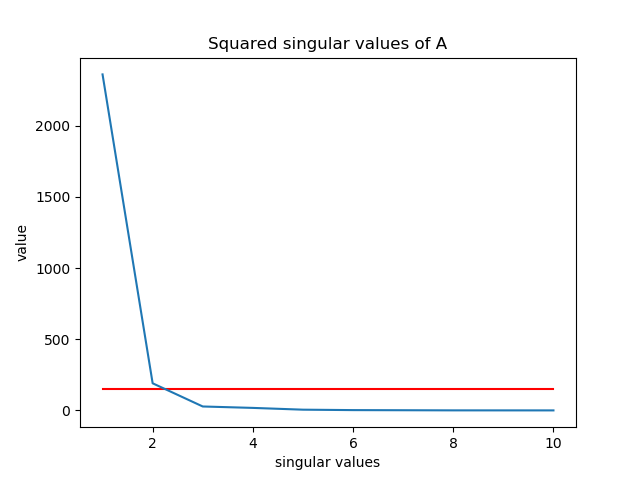
\includegraphics[width=0.5\textwidth]{p5_1.png}
            \caption{squared singular values of A}
            \label{fig.p5_1}
    \end{figure}
    \newpage
    \item [2)] see Figure \ref{fig.p5_2}. See Table \ref{tab.tab2}.
    \begin{figure}[htbp]
        \centering
        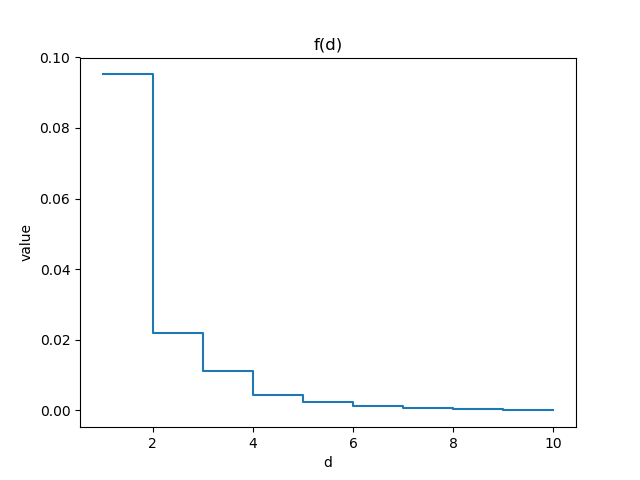
\includegraphics[width=0.5\textwidth]{p5_2.png}
        \caption{f(d)}
        \label{fig.p5_2}
\end{figure}
\end{enumerate}

\end{document}